\documentclass[11pt]{article}

\usepackage{amssymb,amsmath}
\usepackage{times,psfrag,epsf,epsfig,graphics,graphicx,caption}
\usepackage{enumitem}
\usepackage{algorithm}
\usepackage{algorithmic}

\begin{document}
\date{}

\title{PHSX 343: Assignment 4}

\author{William Jardee}

\maketitle


\section*{Problem 1}

\begin{enumerate}[label=\alph*)]
    \item 
    The unprimed frame provides the spacetime interval, as it provides both an inertial frame and has the two events at the same spacial coordinates. 
    
    \item 
    $(c\Delta s)^2 = (c\Delta t)^2 -(\Delta x)^2 - (\Delta y)^2 -(\Delta z)^2$  Metric Equation

    \[(c*32ns)^2 = (c\Delta t)^2 - (13.2m)^2\]
    \[\Delta t = \frac{\sqrt{(c*32\times 10^{-9})^2 + (13.2 m)^2}}{c}\]
    \[\Delta t = 5.440\times 10^{-8}s = 54.40 ns\]
    
 
    \item
    For S': $\Delta t' = 54.40 ns$ and $\Delta x' = 13.2 m$, so $v' = \frac{\Delta x'}{\Delta t'} = \frac{13.2m}{54.40\times 10^{-9} s} = 2.425 \times 10^{8} \frac{m}{s}= 0.8088c$
    
    
    \item
    There are two approaches to this: either take length contraction to not be a thing and get a very confusing solution, or follow what we know from physics 3 and go from there. Since the question doesn't clarify, I will continue by saying that there is length contraction. This assumption leads to the conclusion that the speed of S' as seen by S is the same as the s speed of S as seen by S'. So: $v = -v' = -0.8088c$.\\
    
    
    \item
        \parbox{0}{ 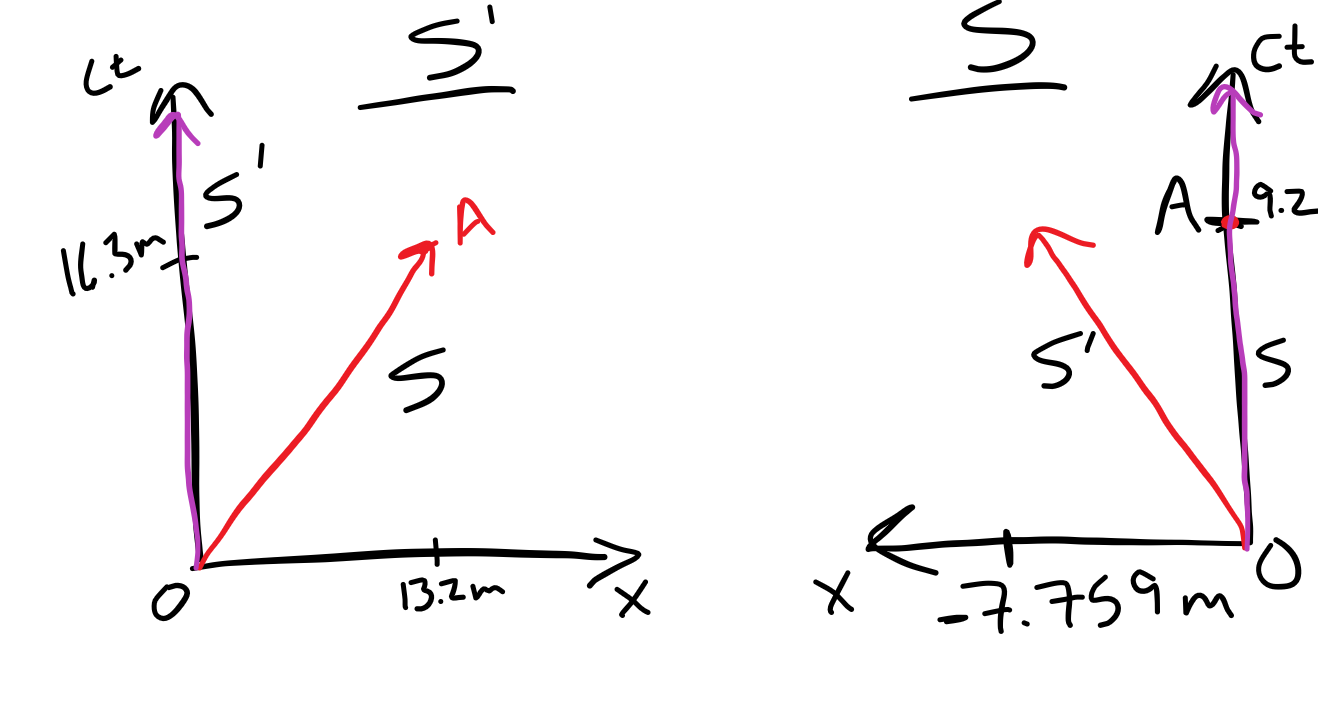
\includegraphics[width = 200pt]{Homework4/homework 4.PNG}}
    
    \item
    When we assume that there is length contraction then Eq. 1.8 works out. If we didn't use than assumption then there is some confusion about which velocity to use, etc.  
    \begin{center} $\Delta t = \frac{\Delta t'}{\sqrt{1-(\frac{v}{c})^2}}$  (Eq. 1.8)
    \end{center}
    Using our values:
    \[\frac{32ns}{\sqrt{1-(\frac{0.8088c}{c})^2}} = \frac{32ns}{\sqrt{1-0.8088^2}} = 54.4ns\]
    So the equation works for our calculations.


\end{enumerate}


\end{document}
